\documentclass[letterpaper,showpacs,prb,preprint]{revtex4}
%\documentclass[letterpaper,showpacs,prb,preprint]{article}\usepackage{graphicx}
\usepackage{epsfig}
\usepackage{subcaption}
%\usepackage{epstopdf}
%\usepackage{dcolumn}% Align table columns on decimal point
\usepackage{bm}% bold math
%\nofiles
\setlength{\textheight}{9in}
\setlength{\footskip}{.5in}
\setlength{\parindent}{1cm}


\begin{document}
\title{Your Title }
\author{Your Name}
\affiliation{ Your School}
\author{Xuan Luo}
\affiliation{ National Graphene Research and Development Center, Springfield, Virginia 22151, USA}
\date{\today}
\begin{abstract}
\setlength{\parindent}{1cm}
We investigated an important thing, blah,....

\end{abstract}

\newpage
\maketitle
\section{Introduction}
With environmental conservation being a key issue in today's society, blah....


$CO_{2 (g)} + H_{2}O_{(l)} \rightleftharpoons H_{2}CO_{3 (aq)}$

$H_{2}CO_{3 (aq)} + H_{2}O_{(l)} \rightleftharpoons HCO_{3 (aq)}^{-} + H_{3}O^{+}_{(aq)} \; \; \; \; \; K_{1} = 2.5 \times 10^{-4}$

$HCO_{3 (aq)}^{-} + H_{2}O_{(l)} \rightleftharpoons CO_{3 (aq)}^{-2} + H_{3}O^{+}_{(aq)} \; \; \; \; \; K_{2} = 4.69 \times 10^{-11}$ 


In Section II, we detailed our methods to perform first-principle calculations. In Sec. III, we present our results on carbon dioxide and graphene configurations.
In Sec. IV, we discuss and compare our results with experimental and other theoretical research. Finally, our conclusion and future work are found in Sec. V.

\section{Method}

\subsection{Computational Details}

We performed first-principle calculations based on Density Functional
Theory (DFT) within the Perdew-Burke-Ernzerhof (PBE) Generalized
Gradient Approximation (GGA) implemented in the ABINIT\cite{gonze2009}
code. We use the Projected Augmented Wave (PAW) method\cite{blochl1994} with
projectors generated with the ATOM code\cite{holzwarth2001}. 
The 2s and 2p shells were considered valence, and a 2s$^{2}$2p$^{2}$ electron configuration was used to generate the PAW potential for carbon; the radius cutoff was 1.0 a.u.. 
Similarly, a 2s$^{2}$2p$^{4}$ electron configuration was used for oxygen with a 1.0 a.u.  radius cutoff.

\subsection{Surface Calculations}

We ran convergence tests on a a primitive graphene unit cell and  blah....

\begin{table}[hpt]
\caption{k-point convergence calculation of primitive cell}
\begin{tabular}{l c}
k-points&Energy (Hartree)\\
\hline
\hline
2 2 1&-1.1553547264E+01\\
4 4 1&-1.1526914325E+01\\
6 6 1&-1.1527320429E+01\\
\textbf{8 8 1}&\textbf{-1.1526901213E+01}\\
10 10 1&-1.1526939441E+01\\
\end{tabular}
\label{kpt1}
\end{table}


\subsection{Molecule Calculations}

We also ran energy convergence for the molecue, blah

\begin{table}[hpt]
\caption{Energy cutoff convergence calculation of carbon dioxide}
\begin{tabular}{l c}
Cutoff&Energy (Hartree)\\
\hline
\hline
40&-3.8002617065E+01\\
42&-3.8002796642E+01\\
\textbf{44}&\textbf{-3.8002846121E+01}\\
46&-3.8002881896E+01\\
\end{tabular}
\label{ecut}
\end{table}

\subsection{Interface Calculations}

Combining the graphene supercell and carbon dioxide molecule, we used the higher energy cutoff value blah

\begin{table}[hpt]
\caption{Vacuum convergence calculation of supercell}
\begin{tabular}{c c}
Vacuum (Bohr)&Energy\\
\hline
\hline
20&-8.3967989472E+01\\
22&-8.3968201443E+01\\
24&-8.3968348218E+01\\
\textbf{26}&\textbf{-8.3968524753E+01}\\
28&-8.3969623865E+01\\
\end{tabular}
\label{vacuum}
\end{table}

Total energy calculations were then run for successful configurations: for the total interface, 
the isolated carbon dioxide molecule, 
and the isolated graphene surface. Adsorption energy was defined by

$E_{ad} = E_{mol+surf} - E_{surf} - E_{mol}$

where $E_{mol+surf}$, $E_{surf}$, and $E_{mol}$ represent the total energies of the interface, graphene surface, and carbon dioxide molecule, respectively. 
From the total energy output data, 
we used the cut3d program to output charge density distributions for the interface, surface, and molecule. 
We then determined the charge transfer in the interface by finding the difference in charge density between the combined materials and the separate constituents. 


$\Delta \rho(r) = \rho_{mol/surf}(r) - \rho_{surf}(r) - \rho_{mol}(r)$

The charge transfer distributions were plotted in OpenDX.

A summary of our convergence data is displayed in Table \ref{total}.


\begin{table}[hpt]
\caption{Total convergence data}
\begin{tabular}{l c  c  c  c}
 &Graphene (primitive)&Graphene (2$\times$2)&Carbon dioxide&Graphene + CO$_{2}$\\
\hline
\hline
Cell parameter (Bohr)&4.6794529438&9.358905888&16$\times$16$\times$16&9.358905888\\
Energy cutoff (Hartree)&38&38&44&44\\
k-points&8 8 1&8 8 1&N/A&4 4 1\\
Vacuum layer (Bohr)&10&26&N/A&26\\
\end{tabular}
\label{total}
\end{table}


\section{Results}

\subsection{General Results}

Graphene forms a hexagonal 2-dimensional lattice. blah
 

\subsection{Adsorption Energies}

We tested several systems, blah,....


\subsection{Atomic Structure}

Figures \ref{figure1} and \ref{figure1} display the four successfully bonded configurations. 
Figure \ref{figure1} shows interfaces between chemically unaltered carbon dioxide molecules and graphene. 
Figure \ref{figure1}a has the carbon dioxide bonded to two diagonal carbons of the hexagonal graphene. 
Figure \ref{figure1}b bonds the carbon dioxide to two carbons with one in between in the graphene unit cell. 
Figure \ref{figure1} shows interfaces between chemically unaltered carbon dioxide and graphene sheets with a single carbon vacancy. 
Figure \ref{figure1}c fills the carbon vacancy in the graphene with an oxygen of the carbon dioxide molecule. 
Figure \ref{figure1}d fills the vacancy with the carbon from carbon dioxide. 
Total energy minima for structures with pure graphene are displayed in Figure \ref{figure1}.

\begin{figure}[ht]
\begin{subfigure}{0.3\textwidth}
\includegraphics [width=\textwidth]{sin.eps}
\includegraphics [width=\textwidth]{cos.eps}
\caption{sin,cos}
\end{subfigure}
\begin{subfigure}{0.3\textwidth}
\includegraphics [width=\textwidth]{asin.eps}
\includegraphics [width=\textwidth]{acos.eps}
\caption{asin,acos}
\end{subfigure}
\begin{subfigure}{0.3\textwidth}
\includegraphics [width=\textwidth]{tan.eps}
\includegraphics [width=\textwidth]{atan.eps}
\caption{tan,atan}
\end{subfigure}
\caption{Demonstration of stacking figures in a row of three subfigures}
\label{figure1}
\end{figure}


\subsection{Charge Density}

Using our total energy calculations, 
we plotted charge transfer in each successful interface. 
Charge densities were printed from the total energy output for the interface, isolated surface, 
and isolated molecule and subtracted to find charge transfer: gain/loss of electrons (Figure \ref{figure1}). 
The red regions represent electron acceptors, and the blue regions represent electron donors. 

Structure \ref{figure1}a had an isosurface scale of -0.007 to 0.005 $e^{-}$/cell volume. 
Structure \ref{figure1}b had an isosurface scale of -0.005 to 0.005 $e^{-}$/cell volume. 
Structure \ref{figure1}c had an isosurface scale of -0.009 to 0.005 $e^{-}$/cell volume. 
Structure \ref{figure1}d had an isosurface scale of -0.002 to 0.005 $e^{-}$/cell volume. 

\section{Discussion}

\subsection{Adsorption Energy}

As shown in somehing....

\subsection{Charge Density}

The visible charge transfer suggests that  blah.

\section{Conclusion}

In summary, we tested the material blah
However, we concluded that  your conclusion

Analysis of charge density distributions showed that

If we were to redo our work, it would be plausible to do something

\newpage

\section{Executive Summary}

Your summary

\newpage
%\smallskip
\bibliography{sample_ref}{}
\bibliographystyle{apsrev}
%\bibliographystyle{naturemag}
%\newcommand{\comment}[1]{}

\end{document}
